\chapter{Analyses}\label{ch:Analyses}
In this chapter, an analysis of the data collected via the methods described in
the previous chapter (Chapter~\ref{ch:Methods}) is given. Firstly, a brief
initial overview is provided, where descriptive statistics of the equilibria
obtained and the overall characteristics of the strategies used is discussed.
Following this, a critical analysis of the \(p\)-thresholds obtained is carried
out. Here, the environmental effects, on the outcome of the game, discussed
include: number and characteristics of opponents; noise; and degeneracy. Then a
large-scale multivariate analysis is executed before considering the reliability
of the collected data. Note, as of writing, the database currently has 
\input{src/database-code/data/se/20_01_2020/entries-in-database.txt}
entries (rows) and a total number of 
\input{src/database-code/data/se/20_01_2020/number-of-tournaments.txt}
tournament sets. 

\section{Initial Analysis}\label{sec:Initial_Analysis}
In this section, all the data (including those games which could be degenerate)
are considered. Taking a brief look at the graphs produced for each set of
tournaments, it can be seen that the main `shapes' obtained are as seen in
Figure~\ref{fig:example_graphs}.

\begin{figure}
    \begin{subfigure}{.45\textwidth}
        \centering
        \includegraphics[width=\textwidth]{folk_thm/single_game/2/0/0.0/main.pdf}
        \caption{An example of a graph with a clear p-threshold point of approximately 0.28. In this game there is no degeneracy and the opponent strategy playing in the tournament was \textit{Inverse}, without noise.}\label{subfig:clear_thresh_plot}
    \end{subfigure}
    \begin{subfigure}{.45\textwidth}
        \centering
        \includegraphics[width=\textwidth]{folk_thm/single_game/6/110/0.0/main.pdf}
        \caption{An example of a graph where the p-threshold is not as clear. Perhaps this is due to a small amount of noise and hence not enough repetitions or stochasticity of the players. In this case the threshold seems to lie in the range [0.1, 0.3]. There is no degeneracy in this game and opponent strategies in the tournament were: \textit{Feld: 1.0, 0.5, 200}; \textit{Cooperator};  \textit{EvolvedLookerUp2\_2\_2}; \textit{Tullock: 11}; and \textit{ZD-GEN-2: 0.125, 0.5, 3}. Again, this tournament was run with no added noise.}\label{subfig:unclear_thresh_plot}
    \end{subfigure}

    \begin{subfigure}{.45\textwidth}
        \centering
        \includegraphics[width=\textwidth]{folk_thm/single_game/5/77/0.0/main.pdf}
        \caption{An example of a graph where the p-threshold is not clear at all due to some (or all) of the games, which were played by the particular tournament set, being degenerate. In this case, the opponent strategies playing in the tournament were: \textit{Random: 0.5}; \textit{Grumpy: Nice, 10, -10}; \textit{Fortress3}; and \textit{Negation}. This tournament had no added noise.}\label{subfig:degenerate_plot}
    \end{subfigure}
    \begin{subfigure}{.45\textwidth}
        \centering
        \includegraphics[width=\textwidth]{folk_thm/single_game/4/60/0.0/main.pdf}
        \caption{An example of a graph where the least probability of defection
        was constant throughout the varying ending probabilities. In this
        particular tournament there was no ending probability in which
        cooperation was beneficial; with the least probability of defection
        equalling the greatest probability of defection at one. Here, the
        opponents were: \textit{AntiCycler}; \textit{\$e\$}; and
        \textit{Stalker: (D,)}.}\label{subfig:constant_plot}
    \end{subfigure}
    \caption{Example graphs obtained from the experiment.}\label{fig:example_graphs}
\end{figure}

This will be discussed further in the next section as follows:
Figures~\ref{subfig:clear_thresh_plot} and~\ref{subfig:constant_plot}, and
general properties of the p-threshold, will be described in
Section~\ref{sec:Analysis_of_the_p-Threshold}; the stochasticity and accuracy
visible in Figure~\ref{subfig:unclear_thresh_plot} will be analysed in
Sections~\ref{subfig:Effects_of_Stochastic_Players}
and~\ref{subsec:Accuracy_of_Thresholds}, respectively; and finally
Figure~\ref{subfig:degenerate_plot}, and degeneracy overall, will be considered
in Section~\ref{subsec:Effects_of_Degeneracy}.

\begin{table}
\centering
\caption{A table of the summary statistics produced from the data of the experiment.}
\label{tab:summary_stats}
\begin{tabular}{lrrrrrr}
\toprule
{} &  experiment\_number &  number\_of\_players &  tournament\_player\_set &  num\_of\_equilibria &  least\_prob\_of\_defection &  greatest\_prob\_of\_defection \\
\midrule
mean &      107364.481228 &           5.435509 &              97.105850 &           1.913727 &                 0.342275 &                    0.459722 \\
std  &       46880.538807 &           1.726832 &              42.619612 &           2.022014 &                 0.469061 &                    0.489564 \\
min  &           0.000000 &           2.000000 &               0.000000 &           1.000000 &                 0.000000 &                    0.000000 \\
25\%  &       72231.000000 &           4.000000 &              65.000000 &           1.000000 &                 0.000000 &                    0.000000 \\
50\%  &      114641.000000 &           6.000000 &             104.000000 &           1.000000 &                 0.000000 &                    0.000000 \\
75\%  &      147396.000000 &           7.000000 &             133.000000 &           3.000000 &                 1.000000 &                    1.000000 \\
max  &      175399.000000 &           8.000000 &             159.000000 &          39.000000 &                 1.000000 &                    1.000000 \\
\bottomrule
\end{tabular}
\end{table}


The summary statistics gained from running the \textit{describe} method of a
pandas database is given in Figure~\ref{tab:summary_stats}. From this, it can be
seen that the number of opponents the \textit{Defector} played against ranged
from one to seven, with an average of four opponents. Also, as expected, the
mean probability of the game ending encountered was 0.5. Observe that, overall,
there were \(175,399\) distinct tournaments played (\textit{experiment\_number}) with a total of 159 distinct sets of strategies (\textit{tournament\_player\_set}). 
Looking now at the statistics for Nash equilibria, it can be seen that a total
of \(823,823\) equilibrium points were calculated in this experiment, with an
average of \(1.914 \approx 2\) equilibria per game. However, observe, at least
one game obtained 39 equilibria which will be explored into later on in this
section. Considering the probabilities of defection within these equilibria,
notice that both the greatest and the least probabilities of defection ranged
from zero to one inclusive with a \(50\)th percentile of zero. But, looking at
the average values, the least probability has a mean of 0.342 and only just
above this, the greatest probability has a mean of 0.460.

Next, further descriptive statistics are calculated for the strategies. This is
to obtain a more in-depth view on the types of strategies randomly chosen to
play and their characteristics. Executing \textit{value\_counts} method on the
column of strategy names, it is observed that the player which appeared the most
times (9 times) is \textit{ZD-GEN-2: 0.125, 0.5, 3}; followed closely by
\textit{Tideman and Chieruzzi} with 7 sets of tournaments. On the other hand 38
out of the 200 strategies playing in this experiment appeared only once.
Running the \textit{value\_counts} method again, but this time on the memory
depths of the strategies found the majority of strategies to have an infinite
memory depth. On the other hand, strategies having no memory or a depth equal to
one were also significant. Considering the stochasticity of players alongside
how many appearances each strategy made yielded the following chart in
Figure~\ref{fig:stochastic_chart}.

\begin{figure}
    \centering
    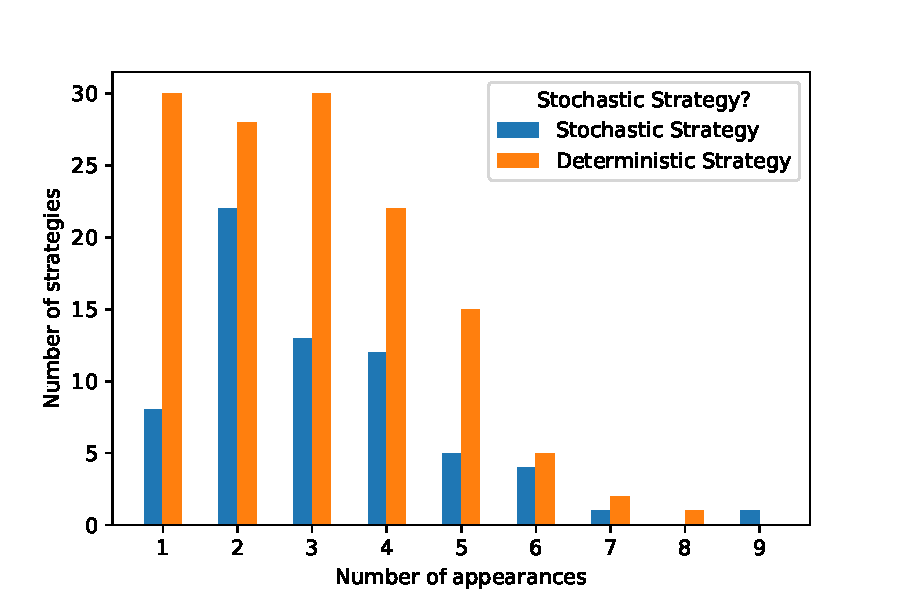
\includegraphics[width=\textwidth]{folk_thm/initial_analysis/strategy_appearances.pdf}
    \caption{A plot to show the ratio of stochastic to deterministic strategies randomly chosen throughout the experiment.}\label{fig:stochastic_chart}
\end{figure}

It is clear that there is a clear bias towards deterministic strategies
in this experiment. However, this is to be expected as running the following
code:
\begin{minted}[frame=lines, framesep=2mm, fontsize=\scriptsize, bgcolor=Cornsilk]{python}
    
    len(axl.filtered_strategies(filterset={"stochastic": True})), 
    len(axl.filtered_strategies(filterset={"stochastic": False}))

    (86, 156)
\end{minted}
it can be seen that over half the strategies coded into the Axelrod library are
classed as deterministic. Looking at Figure~\ref{fig:stochastic_chart} again,
observe, the majority of deterministic strategies were executed either once or
three times. On the other hand, a large proportion of the stochastic strategies
were played twice.

Further, the number of Nash equilibria obtained for each game was analysed and
their distributions with respect to the number of opponents of the
\textit{Defector} plotted. Executing the \textit{value\_counts} method on the
`num\_of\_equilibria' column gave the conclusion that the majority of games
(131773) yielded one Nash equilibria with 28793 games obtaining 3 equilibria.
Also, the maximum number of equilibria yielded, 39, was for one game, which,
doing a search on the database, was found to be a six player game with
noise=0.1. The opponents of the \textit{Defector} were: \textit{Inverse
Punisher}; \textit{Prober}; \textit{PSO Gambler 2\_2\_2 Noise 05};
\textit{Handshake}; and \textit{More Tideman and Chieruzzi}.

Figure~\ref{fig:NE_violinplot} shows the distributions of the number of Nash
equilibria as per the number of players. As can be seen from the plot, the
variance in the number of equilibria increases with the number of players, apart
from when there were 6 players (5 opponents of the defector), where the spread
is maximum. This could be due to the 39 equilibria gained for one game as
discussed in the paragraph above. Looking now at the mean of the distributions,
observe that these are also slightly increasing as the number of players
increase. 

\begin{figure}      
    \centering
    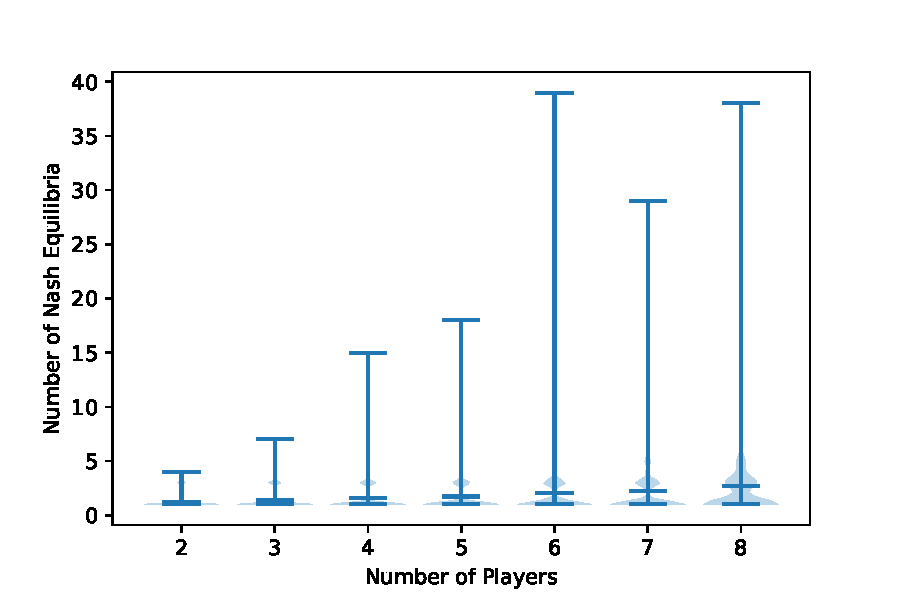
\includegraphics[width=\textwidth]{folk_thm/initial_analysis/player_num_of_equilibria_violinplot.pdf}
    \caption{A violinplot showing the distribution of the number of equilibria obtained for varying number of players.}\label{fig:NE_violinplot}
\end{figure}



\section{Analysis of the p-Threshold}\label{sec:Analysis_of_the_p-Threshold}
In order to analyse the \(p\)-thresholds of the tournaments, two csv files were
created~\footnote{Please see Appendix~\ref{} for the code used to obtain these
files. Also, those tournaments for which all the least probabilities of
defection were greater than 0.5 were omitted - this indicated that regardless of
the ending probability, it was more beneficial to defect.} containing the
minimum, mean, median and maximum probabilities for each set of tournaments.
This was in order to gain as much information as possible from tournaments which
gave graphs as shown in Figure~\ref{fig:less_clear}. That is, tournaments in
which the number of repetitions was not sufficient to omit the `noise' which
could affect the results.

\begin{figure}
    \begin{subfigure}{.3\textwidth}
        \centering
        \includegraphics[width=\textwidth]{folk_thm/single_game/8/157/0.0/main.pdf}
        \caption{This was an eight player tournament with no added noise. The opponent strategies were: \textit{Tester}; \textit{Gradual Killer: (D, D, D, D, D, C, C)}; \textit{Win-Shift Lose-Stay: D}; \textit{Evolved FSM 16}; \textit{Limited Retaliate: 0.1, 20}; \textit{ZD-GEN-2: 0.125, 0.5, 3}; and \textit{Joss: 0.9}.}
    \end{subfigure}
    \begin{subfigure}{.3\textwidth}
        \centering
        \includegraphics[width=\textwidth]{folk_thm/single_game/5/80/0.0/main.pdf}
        \caption{This was a five player tournament with no added noise. The opponent strategies were: \textit{WmAdams}; \textit{Joss: 0.9}; \textit{Yamachi}; and \textit{Stochastic WSLS:\@ 0.05}.}
    \end{subfigure}
    \begin{subfigure}{.3\textwidth}
        \centering
        \includegraphics[width=\textwidth]{folk_thm/single_game/2/24/0.0/main.pdf}
        \caption{This was a two player tournament with no added noise. The \textit{Defector}'s opponent was \textit{Fortress3}.}
    \end{subfigure}
    \caption{Examples of plots where the \(p\)-threshold isn't as clear.}\label{fig:less_clear}
\end{figure}

For clarity, here is a restatement of the definition of a
\textit{\(p\)-threshold}: The maximum probability of the tournament ending for
which cooperation is more beneficial than defection. That is the maximum
probability of the tournament ending for which the probability of defecting is
less than 0.5.

The first csv file created ignored whether a game could be degenerate and, by a
small alteration, the second file contained only the non-degenerate games. This
was in order to help identify whether degeneracy has any effect on the
\(p\)-threshold. Within these files, other than the varying thresholds, the
information about the number of players, tournament strategy set and level of
noise was retained.

Firstly, an exploration into the overall \(p\)-thresholds is given.

\begin{figure}
    \begin{subfigure}{.45\textwidth}
        \centering
        \includegraphics[width=\textwidth]{folk_thm/main_analysis/min_p_thresh.pdf}
        \caption{A plot to show the minimum \(p\)-thresholds.}\label{subfig:min_p_thresh}
    \end{subfigure}
    \begin{subfigure}{.45\textwidth}
        \centering
        \includegraphics[width=\textwidth]{folk_thm/main_analysis/max_p_thresh.pdf}
        \caption{A plot to show the maximum \(p\)-thresholds.}\label{subfig:max_p_thresh}
    \end{subfigure}
    \caption{Plots to show the \(p\)-thresholds for all 1473 sets of tournaments.}\label{fig:min_max_p_thresh}
\end{figure}

Observe, Figure~\ref{subfig:min_p_thresh} shows a `split' in the data, with the
majority of tournaments either having a threshold of less than 0.4 or a
threshold equal to 1. This suggests that for a significant number of
tournaments, it is more beneficial to cooperate if the probability of the
tournament ending is sufficiently small enough (\(\le 3\)). Moreover, there is
a certain number of tournaments in which cooperation is always preferential
over defection. Similar inferences can be made from
Figure~\ref{subfig:max_p_thresh}. On the other hand, looking at the plots in
Figure~\ref{fig:mean_median_p_thresh}, notice that there now appears a
significant number of thresholds falling within the range \([0.5, 0.6]\).
Looking at the tournaments which satisfy the latter observation (see
Figure~\ref{fig:p_mean_middle_plot}), it can be seen that all of these
tournaments had a wide variance. That is, a minimum threshold close to zero and
a maximum threshold close to one. Indeed, looking closer at the plots created
for a few of these tournaments, Figure~\ref{fig:mean_middle_specific}, observe
that there does not seem to be a clear \(p\)-threshold, with the plots having
many peaks.  

\begin{figure}
    \begin{subfigure}{.45\textwidth}
        \centering
        \includegraphics[width=\textwidth]{folk_thm/main_analysis/mean_p_thresh.pdf}
        \caption{A plot to show the mean \(p\)-thresholds.}\label{subfig:mean_p_thresh}
    \end{subfigure}
    \begin{subfigure}{.45\textwidth}
        \centering
        \includegraphics[width=\textwidth]{folk_thm/main_analysis/median_p_thresh.pdf}
        \caption{A plot to show the median \(p\)-thresholds.}\label{subfig:median_p_thresh}
    \end{subfigure}
    \caption{Plots to show the \(p\)-thresholds for all 1473 sets of tournaments.}\label{fig:mean_median_p_thresh}
\end{figure}


\begin{figure}
    \centering
    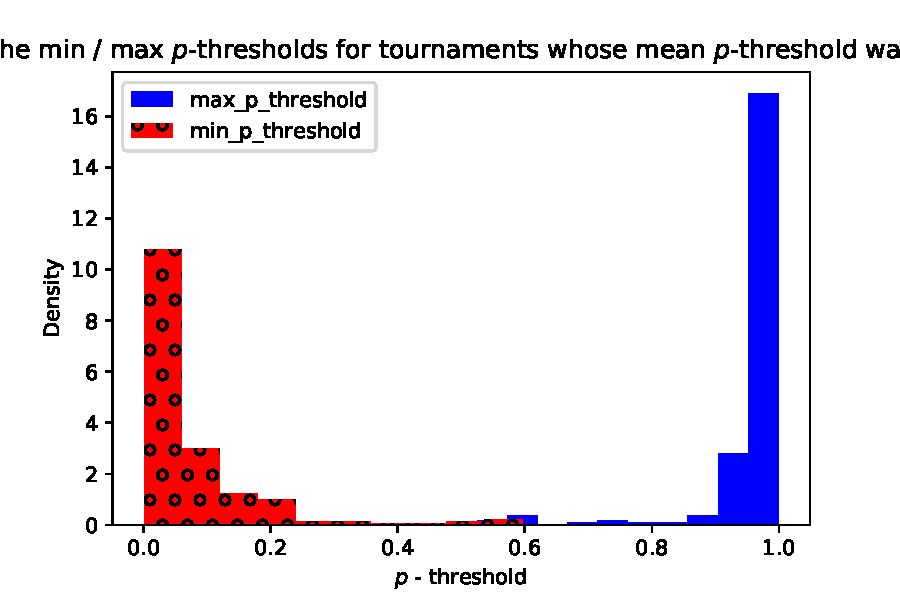
\includegraphics[width=\textwidth]{folk_thm/main_analysis/p_mean_middle_data_plot.pdf}
    \caption{A plot to show the minimum and maximum \(p\)-thresholds for those tournaments which had an mean threshold within the range \([0.5, 0.6]\).}\label{fig:fig:p_mean_middle_plot}
\end{figure}


\begin{figure}
    \begin{subfigure}{0.3\textwidth}
        \centering
        \includegraphics[width=\textwidth]{folk_thm/single_game/6/105/0.2/main.pdf}
        \caption{This plot was obtained from the tournament in which the five
        opponents of the \textit{Defector} were: \textit{RichardHufford};
        \textit{Soft Joss: 0.9}; \textit{Feld: 1.0, 0.5, 200};
        \textit{UsuallyDefects}; and \textit{Handshake}. The tournament also included an additional 0.2 of noise.}
    \end{subfigure}
    \begin{subfigure}{0.3\textwidth}
        \centering
        \includegraphics[width=\textwidth]{folk_thm/single_game/3/35/0.1/main.pdf}
        \caption{This plot represents the, 0.1 noise, tournament with the three players: \textit{Worse and Worse 2}; \textit{Raider}; and, \textit{Defector}.}
    \end{subfigure}
    \begin{subfigure}{0.3\textwidth}
        \centering
        \includegraphics[width=\textwidth]{folk_thm/single_game/3/33/0.5/main.pdf}
        \caption{This plot was produced from the tournament in which the \textit{Defector} was playing \textit{ZD-Extort-2: 0.1111111111111111, 0.5} and \textit{Adaptive Tit For Tat: 0.5}. There was the addition of 0.5 noise within the tournament.}
    \end{subfigure}
    \caption{Example plots of the tournaments where the mean \(p\)-threshold was within the range \([0.5, 0.6]\).}\label{fig:mean_middle_specific}
\end{figure}


\begin{figure}
    \begin{subfigure}{.45\textwidth}
        \centering
        \includegraphics[width=\textwidth]{folk_thm/main_analysis/non_degenerate_min_p_thresh.pdf}
        \caption{A plot to show the minimum \(p\)-thresholds.}\label{subfig:non_degen_min_p_thresh}
    \end{subfigure}
    \begin{subfigure}{.45\textwidth}
        \centering
        \includegraphics[width=\textwidth]{folk_thm/main_analysis/non_degenerate_max_p_thresh.pdf}
        \caption{A plot to show the maximum \(p\)-thresholds.}\label{subfig:non_degen_max_p_thresh}
    \end{subfigure}
    \caption{Plots to show the \(p\)-thresholds for all tournaments which led to non-degenerate games.}\label{fig:non_degen_min_max_p_thresh}
\end{figure}


\begin{figure}
    \begin{subfigure}{.45\textwidth}
        \centering
        \includegraphics[width=\textwidth]{folk_thm/main_analysis/non_degenerate_mean_p_thresh.pdf}
        \caption{A plot to show the mean \(p\)-thresholds.}\label{subfig:non_degen_mean_p_thresh}
    \end{subfigure}
    \begin{subfigure}{.45\textwidth}
        \centering
        \includegraphics[width=\textwidth]{folk_thm/main_analysis/non_degenerate_median_p_thresh.pdf}
        \caption{A plot to show the median \(p\)-thresholds.}\label{subfig:non_degen_median_p_thresh}
    \end{subfigure}
    \caption{Plots to show the \(p\)-thresholds for all tournaments which led to non-degenerate games.}\label{fig:non_degen_mean_median_p_thresh}
\end{figure}

Consider now, the overall \(p\)-threshold for those tournaments which lead to a
non-degenerate game. Comparing
Figures~\ref{subfig:non_degen_min_p_thresh},~\ref{subfig:non_degen_max_p_thresh},~\ref{subfig:non_degen_mean_p_thresh}
and~\ref{subfig:non_degen_median_p_thresh} with Figures~\ref{subfig:min_p_thresh},~\ref{subfig:max_p_thresh},~\ref{subfig:mean_p_thresh}
and~\ref{subfig:median_p_thresh}, respectively, it can be seen that the majority
of thresholds remain the same with only a very small number changing. This could
be due to the number of games that were removed since obtaining the length of
both csv files suggested that only four full tournaments were removed.
The effects of degeneracy will be investigated in more depth in Section~\ref{subsec:Effects_of_Degeneracy}.


\subsection{Effects of the Number of Players}\label{subsec:Effects_of_the_number_of_Players}
In this section, the \(p\)-thresholds will be analysed with respect to the
number of opponents the \textit{Defector} played against. Note, in this section,
only the mean \(p\)-thresholds of games which are non-degenerate will be discussed. 


\begin{figure}
    \centering
    \includegraphics[width=\textwidth]{folk_thm/main_analysis/player_mean_thresh_violinplot.pdf}
    \caption{A violinplot showing the distribution of mean \(p\)-thresholds for each number of opponents.}\label{fig:player_mean_thresh_violinplot}
\end{figure}

From Figure~\ref{fig:player_mean_thresh_violinplot}, it can be seen that the
distributions of the \(p\)-thresholds with respect to the number of players are
approximately the same. The means of the data falls around 0.7 with the main
mode for each number of players being close to 1. Observe, though, that for the
larger group of players (6, 7, 8), the distributions become bimodal with the
second mode around 0.5. This is most significant in the eight player tournaments
however, note that, as of writing, the experiment was still running for eight
player games and hence less data is available currently for this situation.


\subsection{Effects of Stochastic Players}\label{subsec:Effects_of_Stochastic_Players}

In order to analyse the effect of stochastic strategies on the \(p\)-threshold,
tournaments in which these strategies featured are repeated but omitting the
stochastic players to identify any alterations in the results. 




\subsection{Effects of Noise}\label{subsec:Effects_of_Noise}

Here, an analysis on the effects of noise on the \(p\)-threshold is provided.
The addition of noise to a tournament indicates that, with a certain
probability, the action of a particular strategy is
altered~\cite{glynatsi2020meta}. That is, an action of \textit{coop} changes to
\textit{defect} and vice versa.  

\begin{figure}
    \begin{subfigure}{.45\textwidth}
        \centering
        \includegraphics[width=\textwidth]{{folk_thm/main_analysis/0.0noise_mean_p_thresh}.pdf}
        \caption{A plot to show the mean \(p\)-thresholds for all tournaments with no added noise.}\label{subfig:0.0noise_mean_p_thresh}
    \end{subfigure}
    \begin{subfigure}{.45\textwidth}
        \centering
        \includegraphics[width=\textwidth]{{folk_thm/main_analysis/0.1noise_mean_p_thresh}.pdf}
        \caption{A plot to show the mean \(p\)-thresholds for all tournaments with noise = 0.1.}\label{subfig:0.1noise_mean_p_thresh}
    \end{subfigure}

    \begin{subfigure}{.3\textwidth}
        \centering
        \includegraphics[width=\textwidth]{{folk_thm/main_analysis/0.2noise_mean_p_thresh}.pdf}
        \caption{A plot to show the mean \(p\)-thresholds for all tournaments with noise = 0.2.}\label{subfig:0.2noise_mean_p_thresh}
    \end{subfigure}
    \begin{subfigure}{.3\textwidth}
        \centering
        \includegraphics[width=\textwidth]{{folk_thm/main_analysis/0.3noise_mean_p_thresh}.pdf}
        \caption{A plot to show the mean \(p\)-thresholds for all tournaments with noise = 0.3.}\label{subfig:0.3noise_mean_p_thresh}
    \end{subfigure}
    \begin{subfigure}{.3\textwidth}
        \centering
        \includegraphics[width=\textwidth]{{folk_thm/main_analysis/0.4noise_mean_p_thresh}.pdf}
        \caption{A plot to show the mean \(p\)-thresholds for all tournaments with noise = 0.4.}\label{subfig:0.4noise_mean_p_thresh}
    \end{subfigure}

    \begin{subfigure}{.3\textwidth}
        \centering
        \includegraphics[width=\textwidth]{{folk_thm/main_analysis/0.5noise_mean_p_thresh}.pdf}
        \caption{A plot to show the mean \(p\)-thresholds for all tournaments with noise = 0.5.}\label{subfig:0.5noise_mean_p_thresh}
    \end{subfigure}
    \begin{subfigure}{.3\textwidth}
        \centering
        \includegraphics[width=\textwidth]{{folk_thm/main_analysis/0.6noise_mean_p_thresh}.pdf}
        \caption{A plot to show the mean \(p\)-thresholds for all tournaments with noise = 0.6.}\label{subfig:0.6noise_mean_p_thresh}
    \end{subfigure}
    \begin{subfigure}{.3\textwidth}
        \centering
        \includegraphics[width=\textwidth]{{folk_thm/main_analysis/0.7noise_mean_p_thresh}.pdf}
        \caption{A plot to show the mean \(p\)-thresholds for all tournaments with noise = 0.7.}\label{subfig:0.7noise_mean_p_thresh}
    \end{subfigure}
    \begin{subfigure}{.3\textwidth}
        \centering
        \includegraphics[width=\textwidth]{{folk_thm/main_analysis/0.8noise_mean_p_thresh}.pdf}
        \caption{A plot to show the mean \(p\)-thresholds for all tournaments with noise = 0.8.}\label{subfig:0.8noise_mean_p_thresh}
    \end{subfigure}
    \begin{subfigure}{.3\textwidth}
        \centering
        \includegraphics[width=\textwidth]{{folk_thm/main_analysis/0.9noise_mean_p_thresh}.pdf}
        \caption{A plot to show the mean \(p\)-thresholds for all tournaments with noise = 0.9.}\label{subfig:0.9noise_mean_p_thresh}
    \end{subfigure}
    \begin{subfigure}{.3\textwidth}
        \centering
        \includegraphics[width=\textwidth]{{folk_thm/main_analysis/1.0noise_mean_p_thresh}.pdf}
        \caption{A plot to show the mean \(p\)-thresholds for all tournaments with noise = 1.0.}\label{subfig:1.0noise_mean_p_thresh}
    \end{subfigure}
    \caption{Plots to show the mean \(p\)-threshold for varying levels of noise.}\label{fig:noise_mean_p_thresh}
\end{figure}


Figure~\ref{fig:noise_mean_p_thresh} shows the mean \(p\)-thresholds for all
non-degenerate tournaments with the addition of varying probabilities of noise.
Firstly, observe that for those tournaments with the addition of noise at least
0.6
(Figures~\ref{subfig:0.6noise_mean_p_thresh},~\ref{subfig:0.6noise_mean_p_thresh},~\ref{subfig:0.6noise_mean_p_thresh},~\ref{subfig:0.6noise_mean_p_thresh},~\ref{subfig:0.6noise_mean_p_thresh})
the majority of thresholds are equal to one. This is due to the definition of
the parameter noise in the tournaments as described above, That is, there is a
greater chance that the \textit{Defector's} strategy will change to cooperation.
Hence, only tournaments with noise\(\le 0.5\) will be considered. 


\begin{figure}
    \centering
    \includegraphics[width=\textwidth]{folk_thm/main_analysis/noise_mean_thresh_violinplot.pdf}
    \caption{A violinplot showing the distribution of mean \(p\)-thresholds for each level of noise.}\label{fig:noise_mean_thresh_violinplot}
\end{figure}



\subsection{Effects of Degeneracy}\label{subsec:Effects_of_Degeneracy}

\section{Multivariate Data Analysis}\label{sec:MV_Data_Analysis}

\section{Reliability of Data}\label{sec:Reliability_of_Data}

\subsection{Comparison of Databases}\label{subsec:Comparison_of_Databases}

\subsection{Accuracy of Thresholds}\label{subsec:Accuracy_of_Thresholds}